\documentclass[polish,aspectratio=169]{beamer}

% wide screen
% \documentclass[aspectratio=169]{beamer}


%%% YOUR PACKAGES HERE %%%
\usepackage{comment}
\usepackage{hyperref}
\usepackage{biblatex}
\addbibresource{bibliography/bibliography.bib}
\usepackage{subfigure}
\usepackage{graphicx}
\usepackage{geometry}
\usepackage{float}
\usepackage{listings}
\usepackage{xcolor}

% polish language
\usepackage[polish]{babel}
\usepackage{polski}



%%% IMPORT PG PRESENTATION STYLE %%%
% THIS IS GDANSK UNIVERSITY OF TECHNLOGOGY (PG) PRESENTATION TEMPLATE
% Creator: Jan Cychnerski <jan.cychnerski@eti.pg.edu.pl>
% Copyleft 2019


% PG THEME OPTIONS

\usetheme{Boadilla}
\usecolortheme{default}
\usefonttheme{professionalfonts}

% colors

\definecolor{PGBlue}{RGB}{58, 0, 15}
\definecolor{PGRed}{RGB}{193,10,39}
\definecolor{PGSilver}{RGB}{200,200,200}
\definecolor{PGBlack}{RGB}{0,0,0}

% PGBlue
\setbeamercolor{frametitle}{fg=PGBlue}
\setbeamercolor{normal text}{fg=PGBlue}
\setbeamercolor{structure}{fg=PGBlue}
\setbeamercolor{item}{fg=PGBlue}

% PGRed
\setbeamercolor{alerted text}{fg=PGRed}
\setbeamercolor{item projected}{fg=PGRed}

% white
\setbeamercolor{title}{fg=white}
\setbeamercolor{titlelike}{fg=white}
\setbeamercolor{subtitle}{fg=white}

% enumerate and itemize styles

\setbeamertemplate{itemize item}{\bfseries\color{PGRed}\raise1pt\hbox{\donotcoloroutermaths$\bullet$}}
\setbeamertemplate{itemize subitem}{\color{PGRed}\raise0.5pt\hbox{--}}
\setbeamertemplate{itemize subsubitem}{\color{PGRed}\tiny\raise1.5pt\hbox{\donotcoloroutermaths$\bullet$}}

\setbeamertemplate{enumerate item}{\bfseries\color{PGRed}\insertenumlabel.}
\setbeamertemplate{enumerate subitem}{\color{PGRed}\insertsubenumlabel.}
\setbeamertemplate{enumerate subsubitem}{\color{PGRed}\insertsubsubenumlabel.}
\setbeamertemplate{enumerate mini template}{\insertenumlabel}


% disable navigation

\beamertemplatenavigationsymbolsempty

% additional commands

\newcommand*{\vcenteredhbox}[1]{\begingroup
\setbox0=\hbox{#1}\parbox{\wd0}{\box0}\endgroup}

\graphicspath{{pgbeamer/}}


\usepackage{iflang}
\IfLanguageName{polish}{
\newcommand{\pglogobig}{pg-logo-big-pl}
\newcommand{\pglogosmall}{pg-logo-small-pl}
}{
\newcommand{\pglogobig}{pg-logo-big-en}
\newcommand{\pglogosmall}{pg-logo-small-en}
}


% FRAME TITLE LOGO
\addtobeamertemplate{frametitle}{\vcenteredhbox{\includegraphics[height=8mm]{\pglogosmall}}\bfseries}{}


\newcommand{\pgtitleframe}{{
% PG TITLE PAGE

\setbeamercolor{background canvas}{bg=PGBlue}
\setbeamercolor{title}{fg=white}
\setbeamercolor*{date}{fg=white}
\setbeamercolor*{author}{fg=white}

\setbeamertemplate{footline}{}

\begin{frame}[noframenumbering]
\centering
\vspace{1cm}
\includegraphics[height=3cm]{\pglogobig}
\vspace{5mm}
\maketitle
\end{frame}
}}

\newcommand{\pglastframe}{{
% PG LAST PAGE

\setbeamercolor{background canvas}{bg=PGBlue}
\setbeamercolor{title}{fg=white}
\setbeamercolor*{date}{fg=white}
\setbeamercolor*{author}{fg=white}

\setbeamertemplate{footline}{}

\begin{frame}[noframenumbering]
\centering
\vspace{1cm}
\includegraphics[height=5cm]{\pglogobig}
\end{frame}
}}



%%% YOUR OPTIONS HERE %%%

\title[Algorytmy dominowania rzymskiego słabo spójnego]{Analiza algorytmów dla dominowania rzymskiego słabo spójnego}
\subtitle{Analysis of algorithms for weakly connected Roman domination}
\author{inż. Paulina Brzęcka}
\date{\today}

\setbeamercovered{invisible}
\begin{document}

\pgtitleframe

\begin{frame}{Definicja problemu}
    \begin{block}{Definicja}
        Funkcję dominującą rzymską słabo spójną (WCRDF) na grafie \( G \) definiuje się jako taką funkcję dominującą rzymską \( f \colon V(G) \to \{0, 1, 2\} \), dla której zbiór wierzchołków
        \[
        \{ u \in V(G) : f(u) \in \{1, 2\} \}
        \]
        stanowi jednocześnie słabo spójny zbiór dominujący.
        
        \vspace{1em}

        Wagę funkcji \( f \) definiuje się jako:
        \[
        f(V) = \sum_{u \in V} f(u)
        \]

        Liczbą dominowania rzymskiego słabo spójnego grafu \( G \) nazywamy najmniejszą możliwą wagę funkcji \( f \) spełniającej powyższe warunki i oznaczamy ją symbolem:
        \[
        \gamma^{\mathrm{wc}}_R(G)
        \]
    \end{block}
\end{frame}

\begin{frame}{Przykład}
    \begin{figure}
        \centering
        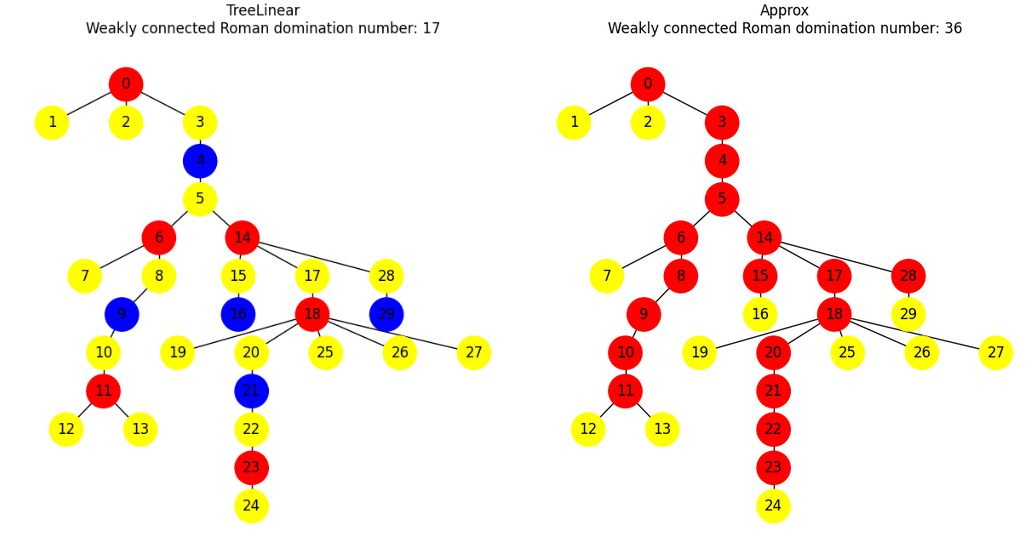
\includegraphics[width=0.9\textwidth]{images/image1.png}
        \caption{Wybrane wyniki dla drzew.}
    \end{figure}    
\end{frame}

\begin{frame}{Cel pracy}
    \begin{itemize}
        \item analiza algorytmów dla dominowania rzymskiego słabo spójnego,
        \item opisanie już istniejących rozwiązań i opracowanie własnych,
        \item analiza i porównanie ich skuteczności,
        \item znalezienie możliwych praktycznych zastosowań.
    \end{itemize}
\end{frame}

\begin{frame}{Pytania badawcze}
    \begin{itemize}
        \item Jakie algorytmy są w stanie znaleźć WCRDF? Które z nich są w stanie znaleźć dodatkowo najmniejszą sumę wag WCRDF?
        \item Czy czas i jakość działania algorytmów będzie uzależniony od klasy grafów?
        \item Czy i jakie algorytmy heurystyczne mogą skutecznie przybliżyć wartość liczby dominowania rzymskiego słabo spójnego w czasie krótszym niż dokładne algorytmy?
        \item Czy hiperparametry algorytmu mrówkowego można dostroić w taki sposób, aby ten algorytm znajdował liczbę dominowania rzymskiego słabo spójnego bliską optymalnej?
    \end{itemize}
\end{frame}

\begin{frame}{Algorytmy}
    \begin{itemize}
        \item brute force - Brute Force,
        \item liniowy dla drzew - TreeLinear,
        \item programowania liniowego 1 - ILP,
        \item programowania liniowego 2 - ILP2,
        \item mrówkowy - AntColony,
        \item aproksymacyjny - Approx,
        \item zachłanny - Greedy.
    \end{itemize}
\end{frame}

\begin{frame}{Algorytm brute force}
    \begin{table}
        \centering
        \begin{tabular}{|p{4cm}|p{10cm}|}
        \hline
        Działanie & Generowanie wszystkich kombinacji przypisań wartości $\{0,1,2\}$ i sprawdzanie każdej pod względem spełnialności definicji WCRDF. Wybór kombinacji o najmniejszej sumie wag.  \\
        \hline
        Złożoność czasowa & $O(3^n \cdot n^2)$  \\
        \hline
        Jakość rozwiązania & Znalezienie optymalnej $\gamma^{\mathrm{wc}}_R(G)$.\\
        \hline
        Opracowanie & Samodzielne  \\
        \hline
        \end{tabular}
        \label{tab:brute_force}
    \end{table}
\end{frame}

\begin{frame}{Algorytm liniowy dla drzew}
    \begin{table}
        \centering
        \begin{tabular}{|p{4cm}|p{10cm}|}
        \hline
        Działanie & Rozpatrywanie drzewa od liści do korzenia i nadawanie wierzchołkom wartości poprzez analizę relacji ojciec-syn i wartości zdefiniowanych parametrów. \\
        \hline
        Złożoność czasowa &  $O(n)$  \\
        \hline
        Jakość rozwiązania & Znalezienie optymalnej $\gamma^{\mathrm{wc}}_R(G)$ dla drzew.\\
        \hline
        Opracowanie & Wraz z promotorką  \\
        \hline
        \end{tabular}
        \label{tab:liniowy}
    \end{table}
\end{frame}

\begin{frame}{Algorytm programowania liniowego 1}
    \begin{table}
        \centering
        \begin{tabular}{|p{4cm}|p{10cm}|}
        \hline
        Działanie & Model programowania liniowego polegający na definiowaniu podgrafu indukowanego i jego drzewa rozpinającego.  \\
        \hline
        Złożoność czasowa & Wykładnicza  \\
        \hline
        Jakość rozwiązania & Znalezienie optymalnej $\gamma^{\mathrm{wc}}_R(G)$.\\
        \hline
        Opracowanie & Na podstawie literatury  \\
        \hline
        \end{tabular}
        \label{tab:ilp}
    \end{table}
\end{frame}

\begin{frame}{Algorytm programowania liniowego 2}
    \begin{table}
        \centering
        \begin{tabular}{|p{4cm}|p{10cm}|}
        \hline
        Działanie & Model programowania liniowego oparty na przepływach.  \\
        \hline
        Złożoność czasowa & Wykładnicza  \\
        \hline
        Jakość rozwiązania & Znalezienie optymalnej $\gamma^{\mathrm{wc}}_R(G)$.\\
        \hline
        Opracowanie & Na podstawie literatury  \\
        \hline
        \end{tabular}
        \label{tab:ilp2}
    \end{table}
\end{frame}

\begin{frame}{Algorytm mrówkowy}
    \begin{table}
        \centering
        \begin{tabular}{|p{4cm}|p{10cm}|}
        \hline
        Działanie & Budowanie rozwiązania poprzez heurystyki i poziom feromonów na wierzchołkach. Następnie sprawdzenie pod względem poprawności WCRDF i wybór najlepszego rozwiązania.  \\
        \hline
        Złożoność czasowa & $O(num\_iterations \cdot num\_ants \cdot n^2)$  \\
        \hline
        Jakość rozwiązania & Znalezienie prawidłowej WCRDF, niekoniecznie optymalnej $\gamma^{\mathrm{wc}}_R(G)$.\\
        \hline
        Opracowanie & Samodzielne  \\
        \hline
        \end{tabular}
        \label{tab:mrowkowy}
    \end{table}
\end{frame}

\begin{frame}{Algorytm aproksymacyjny}
    \begin{table}
        \centering
        \begin{tabular}{|p{4cm}|p{10cm}|}
        \hline
        Działanie & Znajdowanie zbioru dominującego spójnego w grafie przy użyciu programowania liniowego. Następnie wierzchołkom zbioru dominującego przypisanie wartości 2.  \\
        \hline
        Złożoność czasowa & Wykładnicza  \\
        \hline
        Jakość rozwiązania & Znalezienie prawidłowej WCRDF, niekoniecznie optymalnej $\gamma^{\mathrm{wc}}_R(G)$. Algorytm $2(1 + \varepsilon)(1 + \ln(\Delta - 1))$-aproksymacyjny.\\
        \hline
        Opracowanie & Na podstawie literatury  \\
        \hline
        \end{tabular}
        \label{tab:aproksymacyjny}
    \end{table}
\end{frame}

\begin{frame}{Algorytm zachłanny}
    \begin{table}
        \centering
        \begin{tabular}{|p{4cm}|p{10cm}|}
        \hline
        Działanie & Algorytm rozpoczyna od przypisania wartości 2 wierzchołkowi o największym stopniu oraz zabezpieczenia jego sąsiadów. Następnie, dopóki istnieją wierzchołki niechronione (czyli z przypisaną wartością 0), wybierany jest wierzchołek $v$, który dominuje jak największą liczbę sąsiadów. \\
        \hline
        Złożoność czasowa & $O(n^2)$ - grafy rzadkie, $O(n^3)$ - grafy gęste  \\
        \hline
        Jakość rozwiązania & Znalezienie prawidłowej WCRDF, niekoniecznie optymalnej $\gamma^{\mathrm{wc}}_R(G)$.\\
        \hline
        Opracowanie & Samodzielne  \\
        \hline
        \end{tabular}
        \label{tab:zachlanny}
    \end{table}
\end{frame}

\begin{frame}{Wyniki}
    \begin{figure}
        \centering
        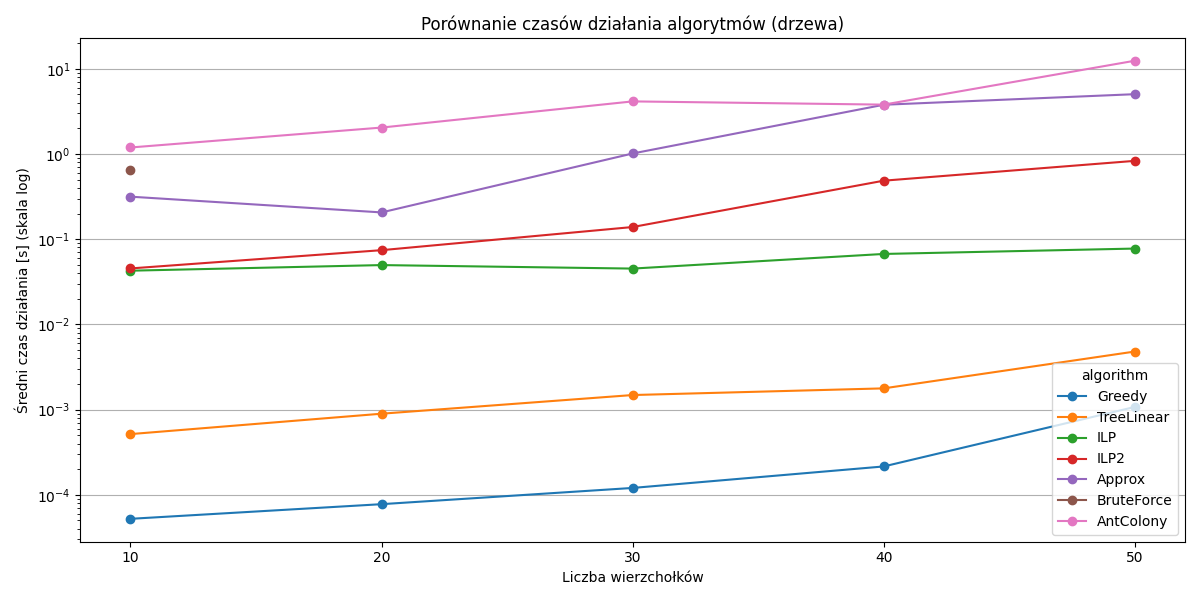
\includegraphics[width=1\textwidth]{images/trees.png}
        \caption{Porównanie czasów działania algorytmów - grafy drzewiaste.}
    \end{figure}    
\end{frame}

\begin{frame}{Wyniki}
    \begin{figure}
        \centering
        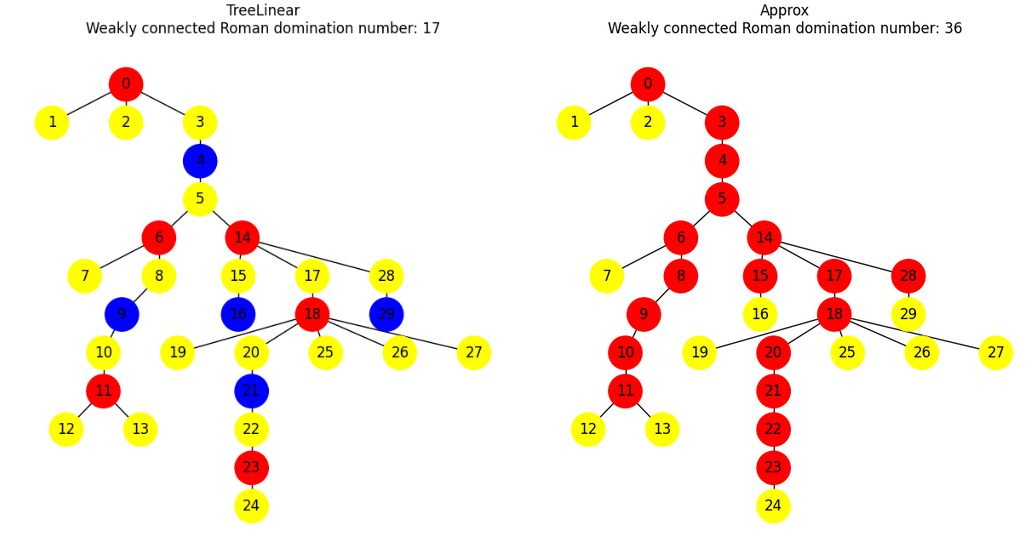
\includegraphics[width=0.9\textwidth]{images/image1.png}
        \caption{Wybrane wyniki dla drzew.}
    \end{figure}    
\end{frame}

\begin{frame}{Wyniki algorytmu aproksymacyjnego}
    \begin{figure}
        \centering
        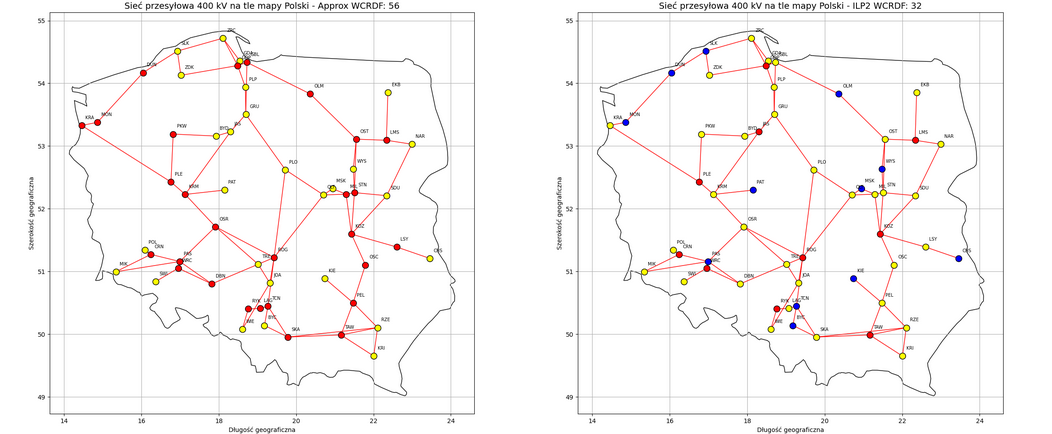
\includegraphics[width=1\textwidth]{images/image.png}
        \caption{Porównanie algorytmów przybliżonych.}
    \end{figure}    
\end{frame}

\begin{frame}{Wyniki algorytmów przybliżonych}
    \begin{figure}
        \centering
        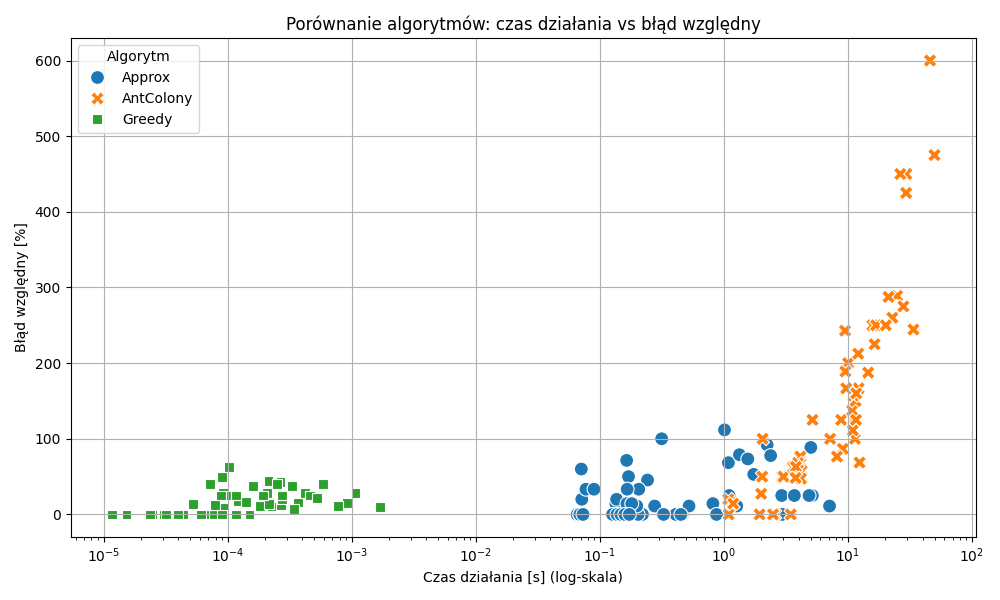
\includegraphics[width=0.8\textwidth]{images/alorithms.png}
        \caption{Porównanie algorytmów przybliżonych.}
    \end{figure}    
\end{frame}

\begin{frame}{Zastosowania praktyczne}
    \begin{figure}
        \centering
        \includegraphics[width=1\textwidth]{images/image2.png}
        \caption{Rozmieszczenie zabezpieczeń sieci energetycznych.}
    \end{figure}    
\end{frame}

\begin{frame}{Wnioski}
\begin{itemize}
    \item udało się odpowiedzieć na wszystkie pytania badawcze,
    \item konieczność doboru właściwego algorytmu do rodzaju lub klasy grafu:
    \begin{itemize}
        \item np. TreeLinear dla drzew, ILP2 dla grafów gęstych, Greedy dla dużych instancji.
    \end{itemize}
    \item algorytmy heurystyczne (Greedy, Approx) zapewniają szybkie i dobre przybliżenia,
    \item słaba jakość rozwiązań algorytmu mrówkowego - niezalecane w tej implementacji,
    \item wskazano potencjalne zastosowania praktyczne (np. sieci energetyczne, społeczne) - potwierdzono zasadność modelu WCRDF.
\end{itemize}
\end{frame}


\begin{frame}{Dalsze kierunki badań}
    \begin{itemize}
        \item implementacja i testy potencjalnych ulepszeń dla algorytmu zachłannego,
        \item rozszerzenie testów na inne klasy, jak i na inne wielkości grafów,
        \item podniesienie jakości wyników algorytmu mrówkowego, między innymi poprzez inną implementację heurystyki lokalnej oraz strategii feromonowej,
        \item opracowanie algorytmów dokładnych, rozwiązywalnych w czasie wielomianowym dla innych klas grafów,
        \item weryfikacja i przełożenie teoretycznych rozważań na temat praktycznych zastosowań tego problemu na praktyczną analizę i realizację.
    \end{itemize}
\end{frame}

\begin{frame}[c]
    \centering
    \Huge \textbf{Dziękuję za uwagę!}
\end{frame}

% \setbeamercovered{transparent}
% \begin{frame}{Bibliografia}
%     \nocite{*}
%     \printbibliography
% \end{frame}

\pglastframe

\end{document}